% Chapter 5
\chapter{Empirical Results} % Main chapter title
\label{Chapter5} 

This chapter presents the empirical results of the financial-environmental attribution framework, analyzing and contrasting the environmental pressures financed by the financial systems of the United States and the Euro area. By mapping macro-financial asset allocations to physical environmental flows, the analysis reveals how distinct institutional structures and geographic investment strategies drive global environmental profiles. 

The chapter is structured as follows: Section \ref{sec:6.1} explores the structural evolution of financial exposures across institutional categories and real-economy agents, establishing the macroeconomic foundations of both systems. Section \ref{sec:6.2} evaluates financed emissions, decomposing portfolio footprints through regional scenarios and comparing them against traditional production- and consumption-based accounting benchmarks. Finally, Section \ref{sec:6.3} expands the attribution framework beyond carbon metrics to evaluate multi-dimensional ecosystem pressures, focusing on land use, blue-water consumption, and upstream resource extraction.

\section{Financial Exposures Across Institutions and Economic Agents}
\label{sec:6.1}

Figure \ref{fig:total_exp_fi} illustrates the evolution of total financial institution exposure in the US and the EZ, revealing substantial differences in the financial structures of the two regions. The Euro area features a "bank-based" system, where monetary financial institutions are the predominant source of economic financing. In contrast, the proportion of finance channeled through non-bank institutions is significantly higher in the US. This aligns with the well-documented characterization of the US as a "market-based" system, where funds are raised primarily through securities markets \citep{de_fiore_bank_2005, bats_bank-based_2020}. \textcite{de_fiore_bank_2005} attributes these structural differences to the lower availability of public information regarding firms' creditworthiness in the Euro area, coupled with the higher efficiency of its banks in acquiring this information. Recognizing these distinct financial frameworks is crucial for analyzing how exposure evolves over time. For example, research indicates that bank-oriented systems are more susceptible to financial crises and systemic risks than market-based systems, suffering higher rates of bank defaults during economic downturns \citep{gambacorta_financial_2014, bats_bank-based_2020}. This inherent vulnerability helps explain the severe post-2008 contraction of banking assets in the Euro area, which did not recover to pre-crisis levels until after 2020. In contrast, the US financial system experienced only a temporary slowdown and avoided comparable systemic deterioration.

Another noticeable difference between the US and the EZ is the size of pension fund assets under management. While pension fund exposure in the Euro Area has remained relatively limited over time, in the United States pension funds have consistently been as a large and important channel of financial intermediation. This gap largely reflects the prevalence of two distinct pension systems across the regions: pay-as-you-go (PAYG) and capital-funded schemes. PAYG systems, where current contributions are used to finance current retirement benefits, remain dominant in the Euro Area, particularly in populated countries such as Germany, Italy, and France \citep{van_der_zwan_financialisation_2017}. In contrast, the US system relies more heavily on capital-funded pensions, in which workers’ contributions are invested in financial markets and retirement benefits are financed through accumulated returns. Combined with a relatively flexible regulatory environment that permits higher exposure to equities and alternative assets, this structure has enabled substantial asset accumulation over time. Moreover, US pension fund growth has been significantly supported by strong equity market performance, particularly the expansion of the technology sector over the past two decades \citep{andonov_pension_2017}.

Lastly, the activity level of Other Financial Institutions, a common proxy for the shadow banking sector, is not only substantial but has also experienced considerable growth in both regions. As defined in Section \ref{sec:fi_def}, this category includes issuers of asset-backed securities (ABS) and special purpose vehicles (SPVs) that facilitate the securitization process. Prior to 2008, OFI exposure even exceeded that of the traditional banking sector in the US, illustrating the buildup of unregulated securitization that is widely recognized as a primary catalyst for the 2008-2009 Global Financial Crisis \citep{brunnermeier_deciphering_2009}. In the Euro area, a post-crisis substitution effect emerged: the contraction of the traditional banking sector was offset by the expanding activities of the shadow banking sector. However, this growth trajectory has largely stagnated since 2017. This plateau can be primarily attributed to the gradual recovery of traditional bank lending capacities and the introduction of stricter regulatory frameworks aimed at reducing shadow banking risks \citep{european_systemic_risk_board_eu_2018}.

\begin{figure}[h]
    \centering
    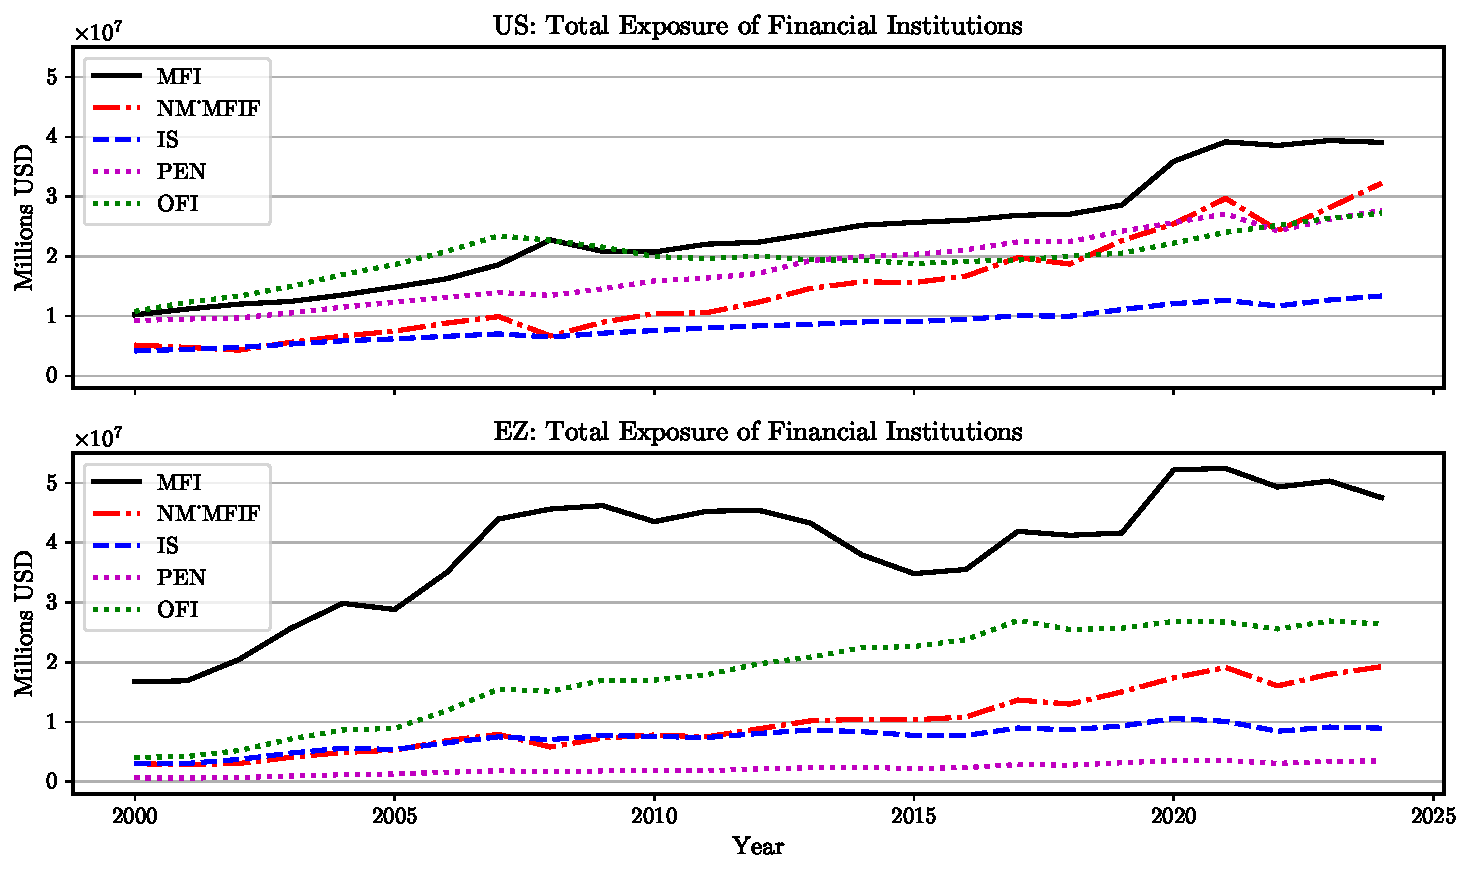
\includegraphics[width=1\textwidth]{Figures/FI_TotalExposure_US_vs_EZ_Institutions.pdf}  
    \caption{Total exposure of Financial Institutions: US and EZ}
    \label{fig:total_exp_fi}
\end{figure}

Figure \ref{fig:total_exp_agent} illustrates which real-economy sectors are financed by regional financial systems. Because these real-economy agents directly impact the environment, identifying them clarifies the core drivers of environmental pressures linked to financing activities. In the US, domestic corporations have consistently remained the largest debt holders. Prior to 2008, both households and the corporate sector received equal funding from financial institutions and experienced a decade of rapid expansion. Following the financial crisis, however, stricter regulations largely halted funding to the household sector. Similarly, the corporate sector was the primary recipient of funding in the Euro area until 2012, marking the peak of the Eurozone debt crisis. Since then, Eurozone financial corporations have increasingly redirected their funding flows outward to foreign markets.

We can also see a divergence in how government debt is financed across the two regions. In the US, the financial system is a massive internal funding engine for the government. This reflects the role of US Treasuries as a foundational safe asset; under post-2008 frameworks like Basel III's Liquidity Coverage Ratio (LCR), domestic institutions face strict requirements to hold High-Quality Liquid Assets (HQLA) to ensure liquidity, driving massive captive demand for government debt \citep{he_agency_2022}. Conversely, Eurozone internal government financing has remained notably stagnant since the 2012 debt crisis. Academic literature on the "bank-sovereign nexus", often called the 'doom loop', helps explain this stagnation. During the crisis, as government debt lost value, the domestic banks holding that debt faced insolvency, which in turn forced governments deeper into debt to rescue them \citep{alogoskoufis_regulating_2018, hristov_macroprudential_2021}. Post-crisis efforts have sought to discourage European financial institutions from over-concentrating in domestic sovereign debt to mitigate this systemic risk \citep{soenen_drivers_2020}. Furthermore, the European Central Bank's prolonged era of negative interest rate policies depressed domestic yields, driving Eurozone banks to search for yield and increasingly redirect their lending flows outward across borders \citep{andreeva_negative_2023}.

\begin{figure}[h]
    \centering
    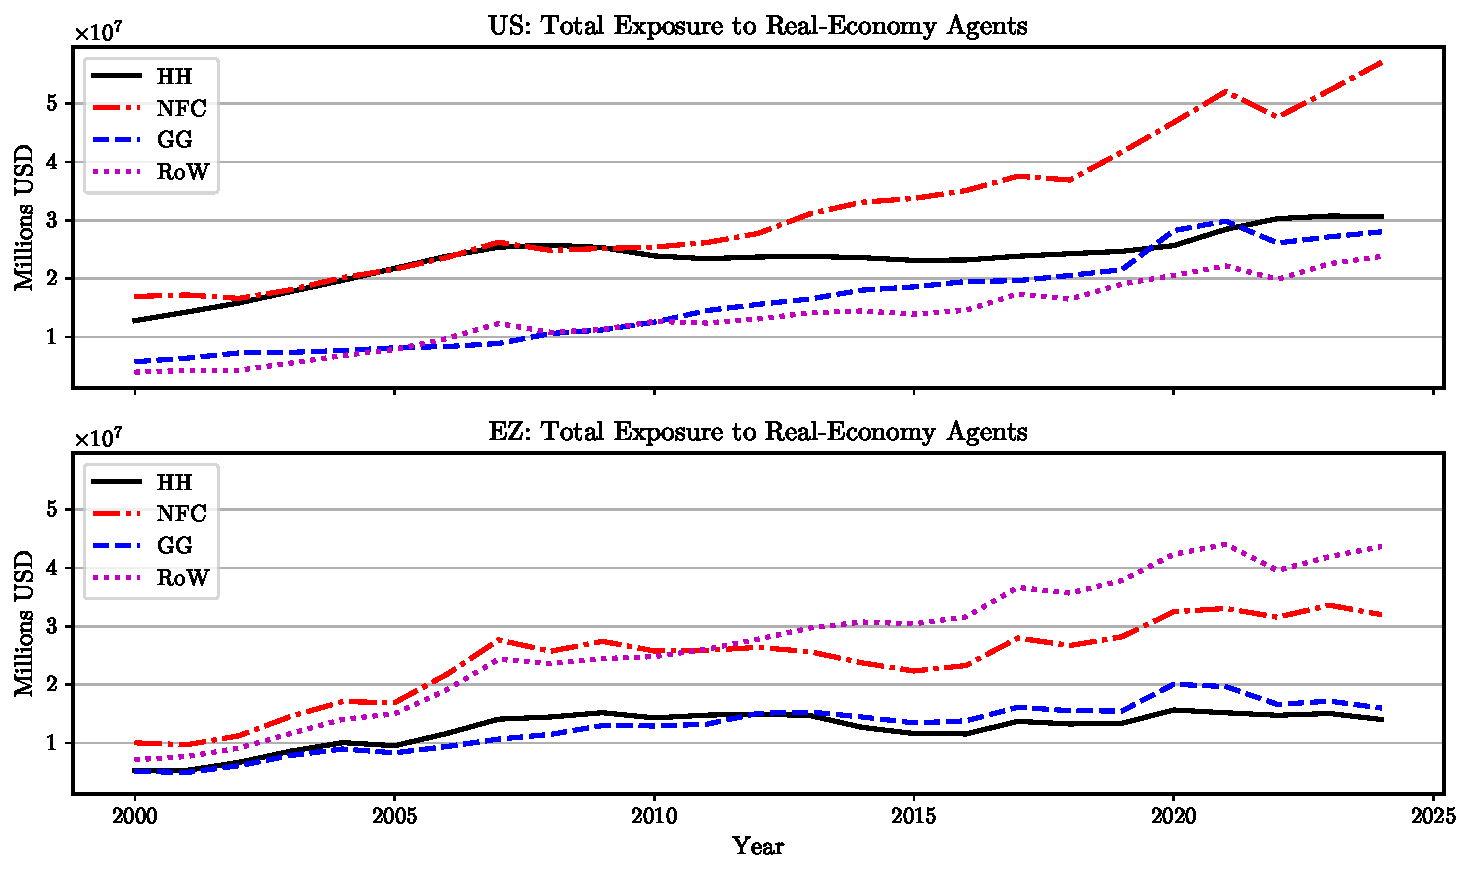
\includegraphics[width=1\textwidth]{Figures/FI_TotalExposure_US_vs_EZ_Agents.pdf}
    \caption{Total exposure to Real-Economy Agents: US and EZ}
    \label{fig:total_exp_agent}
\end{figure}

Overall, the total exposure of the financial system has been larger in the US compared to the Eurozone for most of the observed period (see Figure \ref{fig:total_exp}). While both regions followed similar growth trajectories early on, a significant divergence emerged post-2020, with US exposure accelerating faster. At the end of 2024, the exposure of financial system in the US was 139.6 trillion USD versus 105.7 trillion USD in the EZ. Regarding portfolio composition, the US financial system has consistently maintained a strong domestic focus, allocating over 80\% of its exposure to domestic sectors. In contrast, the Eurozone exhibits a much higher propensity to finance foreign agents, with the RoW sector expanding to account for roughly 40\% of its total exposure by the end of the period.  

\begin{figure}[h]
    \centering
    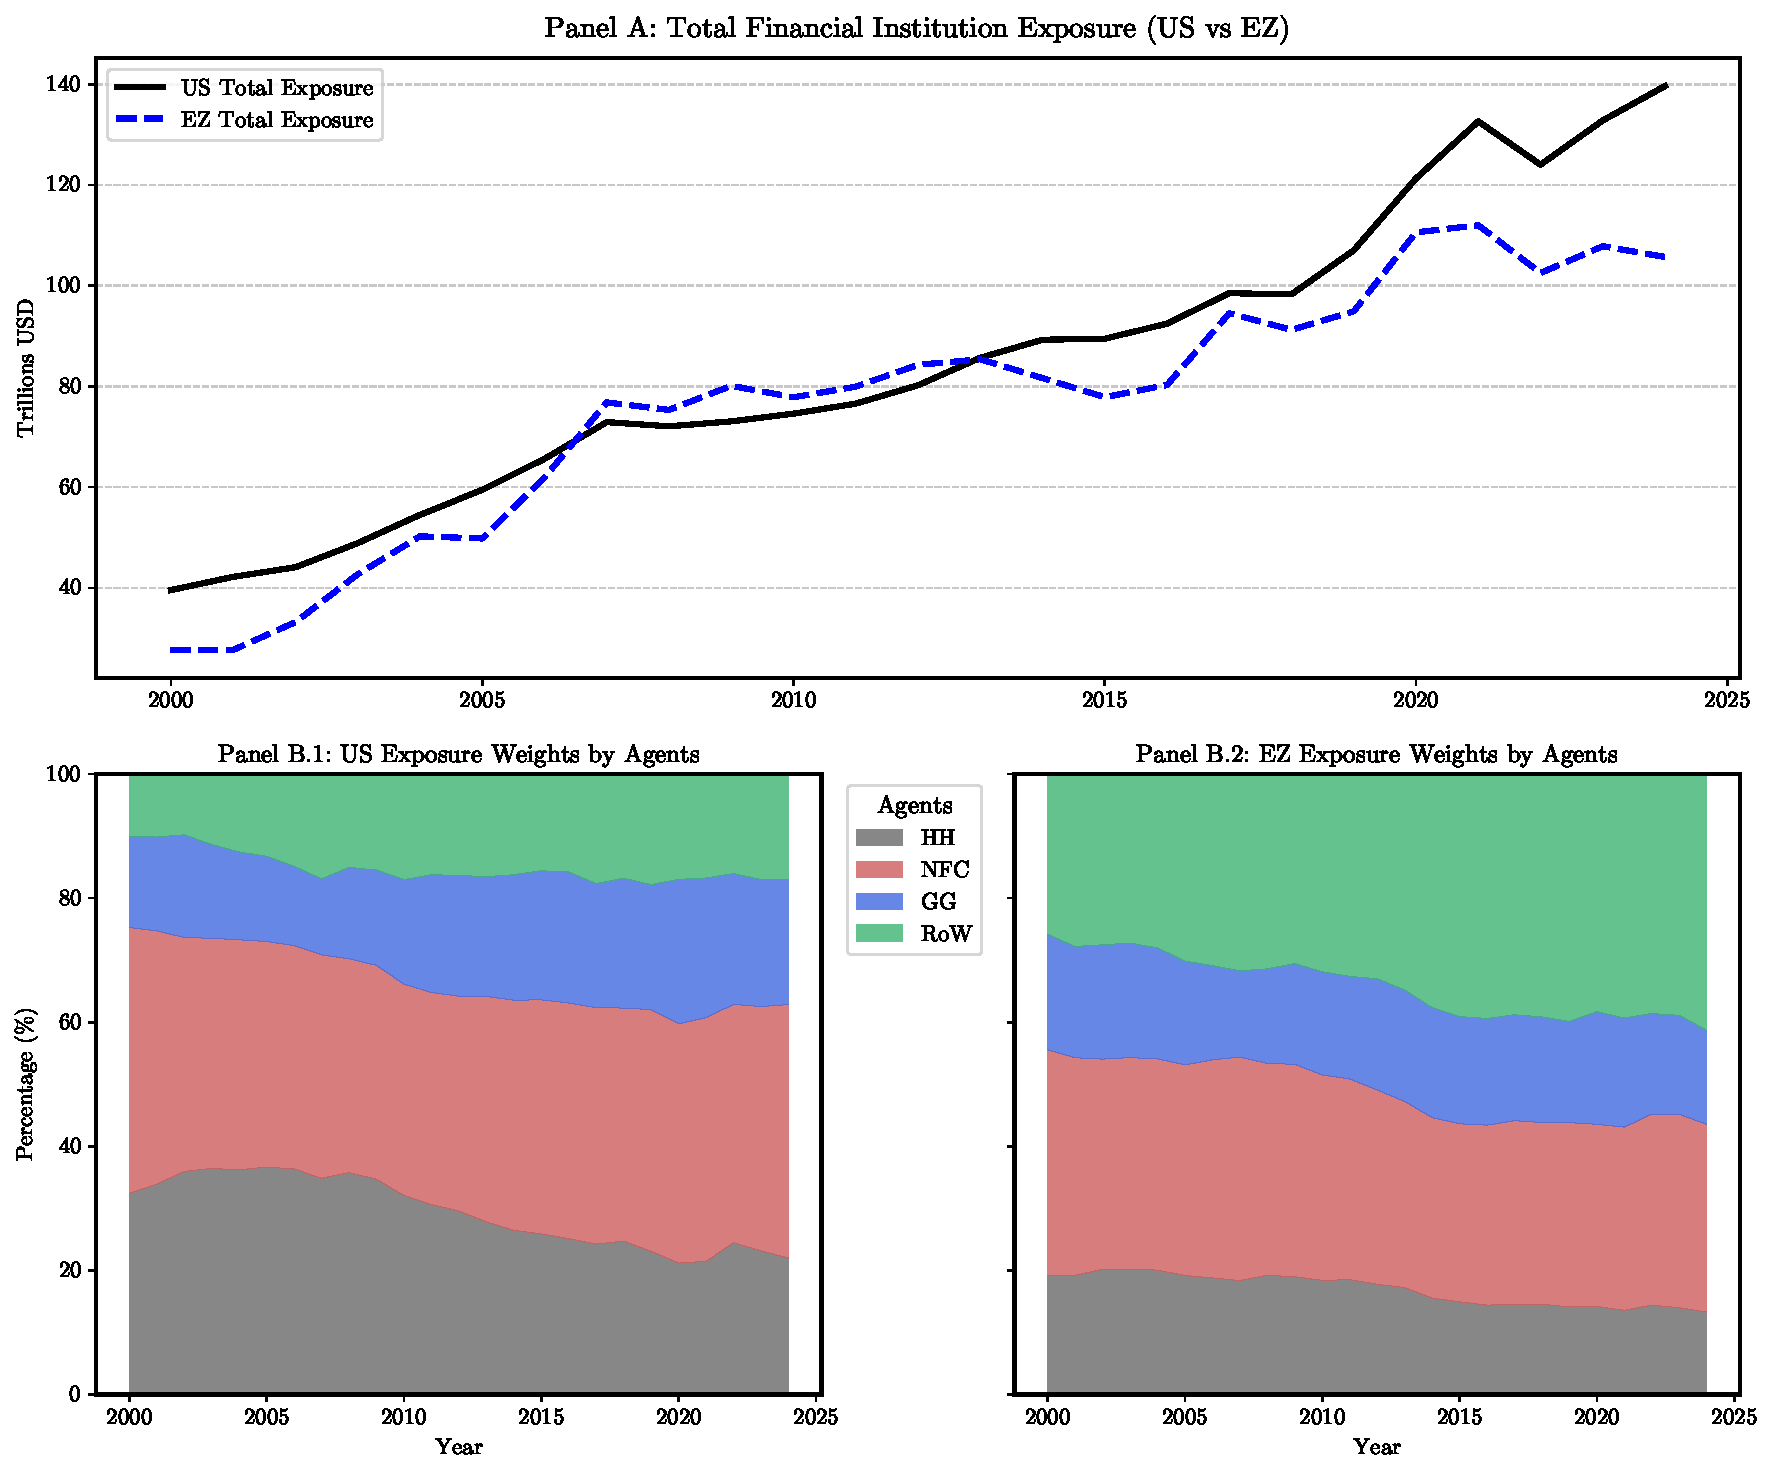
\includegraphics[width=1\textwidth]{Figures/US_vs_EU_Exposure_and_Weights.pdf}
    \caption{Total exposure of the whole financial system and exposure weights by agents}
    \label{fig:total_exp}
\end{figure}

\section{Financed Emissions}
\label{sec:6.2}

\subsection{Carbon Intensity}

The remaining component in calculating total financed emissions in Equation \ref{eq:financed_emis_fi} is the carbon intensity of real-economy agents, defined as the ratio of GHG emissions to their total financial claims ($CI_{k,t}=\frac{E_{k,t}}{TC_{k,t}}$). Because carbon intensity is a ratio, fluctuations can be driven by either numerator effects (changes in absolute emissions) or denominator effects (expansions or contractions in total financial claims). While the following analysis focuses on the resulting intensity trajectories, a full temporal decomposition of the absolute emissions and total claims driving these trends is provided in Appendix \ref{Appendix D:Decompostion}. 


Figure \ref{fig:intensity_dom} reports the carbon intensity of domestic agent groups in the US and the EZ. Over the past two decades, this intensity has steadily declined for all agents across both regions. The government sector consistently exhibits the lowest values, as its associated emissions are primarily confined to public administration activities. By 2022, government carbon intensity stood at approximately 3 $\text{tCO}_2\text{e}$ per million USD for the US, and 3.7 $\text{tCO}_2\text{e}$ per million USD for the Euro area.

The household sector also demonstrates a relatively low carbon intensity that is highly comparable between the two regions. In the US, household intensity dropped significantly from 45.4 $\text{tCO}_2\text{e}$ per million USD in 2000 to 10.7 $\text{tCO}_2\text{e}$ per million USD in 2022. The EZ followed a parallel trajectory, falling from 54.1 $\text{tCO}_2\text{e}$ per million USD down to 14.5 $\text{tCO}_2\text{e}$ per million USD over the same timeframe.

Non-financial corporations consistently exhibit the highest carbon intensity among domestic agents, though these levels have dropped significantly to bridge the gap with other sectors. In the US, the decline has been remarkably steady at roughly 5\% year-over-year, reaching 45.1 $\text{tCO}_2\text{e}$ per million USD by 2022. The EZ, however, demonstrates two distinct phases: a rapid pre-2008 reduction of about 10\% annually, fueled by the expansion of financial assets, followed by a marked slowdown to a 2.5\% annual decline, resulting in an intensity of 52.9 $\text{tCO}_2\text{e}$ per million USD in 2022.
 
\begin{figure}[h]
    \centering
    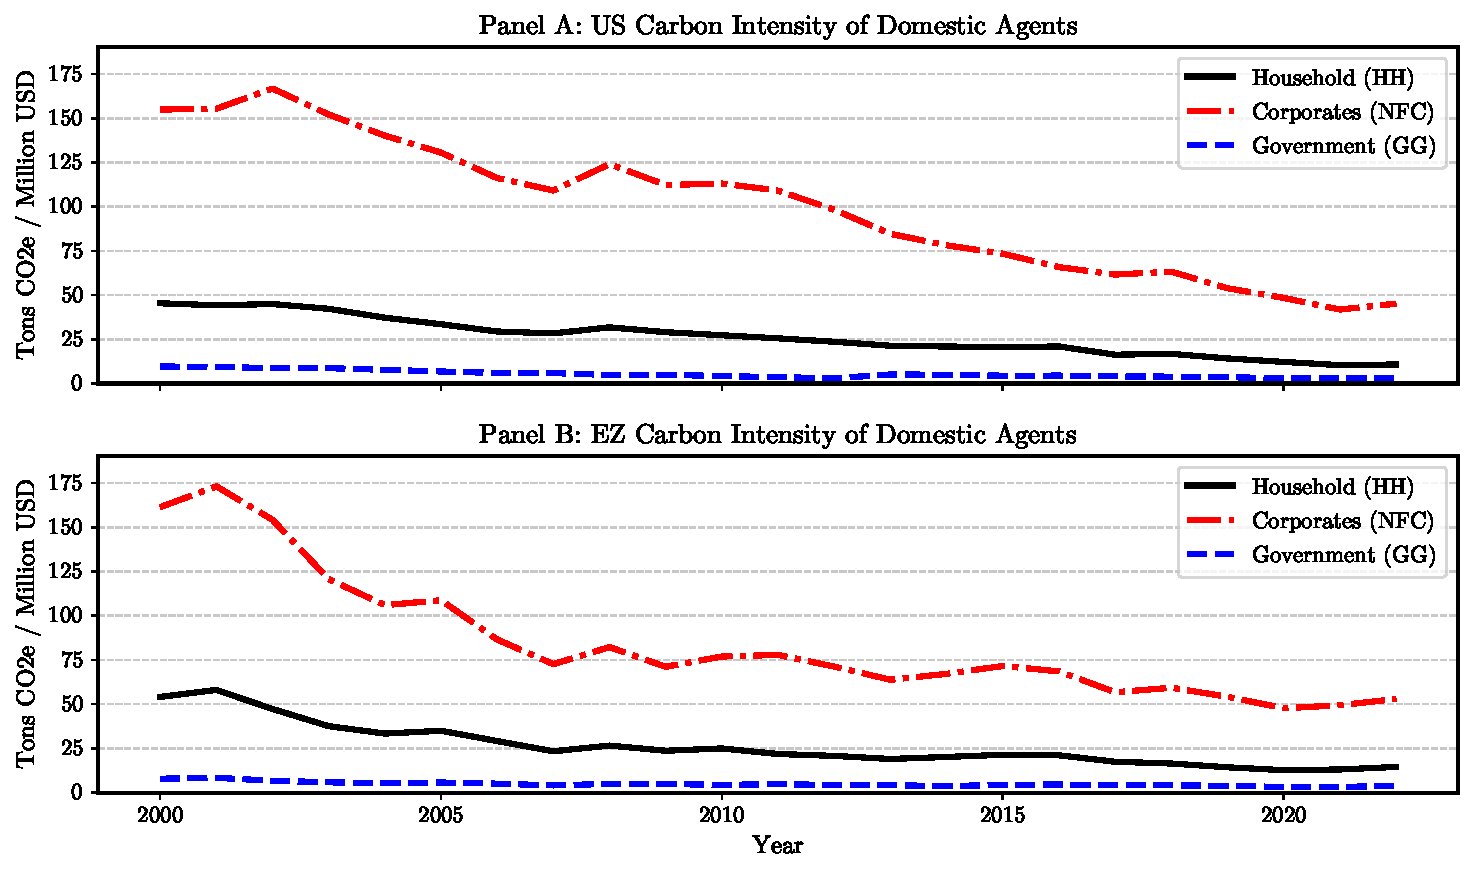
\includegraphics[width=1\textwidth]{Figures/Compare_Domestic_Intensity.pdf}
    \caption{Carbon Intensity of Domestic Agents}
    \label{fig:intensity_dom}
\end{figure}

Figure \ref{fig:intensity_row} presents the carbon intensity of the Rest of the World sector. To assess the robustness of these estimates, I construct alternative regional coverage scenarios: RoW1 corresponds to developed economies (including Europe, North America, and the Japan-Pacific region); RoW2 incorporates emerging economies with available claim information from the OECD (Brazil, India, Mexico, Russia, and Türkiye); and RoW3 expands this coverage to include China, reflecting its leading global position in both financial claims and total emissions.

For both the US and the EZ, the inclusion of emerging economies (RoW2) increases the RoW carbon intensity by approximately 20 $\text{tCO}_2\text{e}$ per million USD, while the further addition of China (RoW3) adds an additional 20 $\text{tCO}_2\text{e}$ per million USD. This disproportionate increase suggests that despite its massive debt levels, China's relative emissions remain exceptionally high. Consequently, financial institutions whose foreign exposures are concentrated in developed countries will benefit from lower portfolio carbon intensities, whereas those diversifying into emerging markets and China will incur significantly higher financed emissions. By 2022, the RoW3 carbon intensity for both the US and EZ reached approximately 60 $\text{tCO}_2\text{e}$ per million USD, ultimately surpassing the intensity of domestic non-financial corporations (NFCs) in both regions.

\begin{figure}[h]
    \centering
    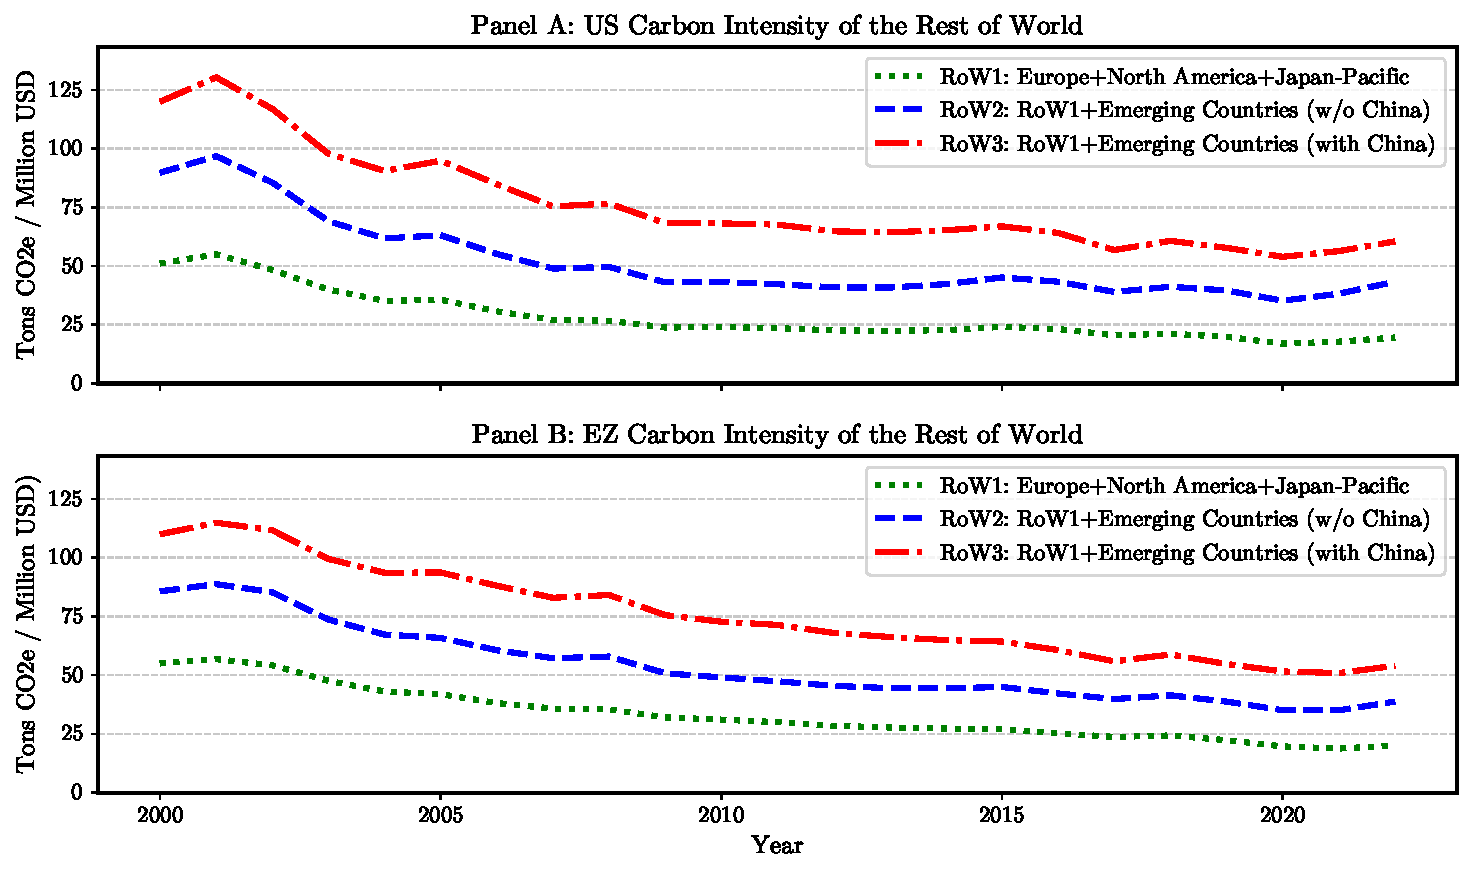
\includegraphics[width=1\textwidth]{Figures/Compare_RoW_Intensity.pdf}
    \caption{Carbon Intensity of the Rest of World}
    \label{fig:intensity_row}
\end{figure}

\subsection{System-wide financed emissions}

Figure \ref{fig:total_financed_emis} summarizes total financed emissions of the US and the Euro area across alternative RoW scenarios. The definition of RoW regions has a sizeable impact on total financed emissions, particularly for financial systems with larger foreign exposures, such as the Euro area.

The US, with its larger financial system and higher domestic corporate carbon intensity prior to 2015, initially accounts for higher financed emissions. After 2015, however, the gap narrows as foreign exposures become increasingly important. Under the broadest RoW3 scenario, which includes emerging markets and China, Euro area financed emissions surpass those of the US in recent years.

Taking RoW1 as the base-case scenario, where foreign exposures are restricted to developed markets, total financed emissions reach $2,946.8$ million tCO$_2$e for the US and $2,739.9$ million tCO$_2$e for the Euro area. Under RoW3, these estimates increase to $3,761.5$ million tCO$_2$e and $4,082.4$ million tCO$_2$e, respectively. This corresponds to an increase of approximately 28\% for the US and 49\% for the Euro area relative to RoW1, highlighting the stronger sensitivity of Euro area financed emissions to assumptions about foreign-market exposure.

These differences depend on the extent to which financing flows spill over into more carbon-intensive emerging markets and China. According to a publication by the Federal Reserve, U.S. residents' holdings of emerging market long-term securities account for approximately one-third of their total foreign holdings of long-term securities\footnote{Source: The Federal Reserve, available at \url{https://www.federalreserve.gov/releases/efa/international-portfolio-investment-figure4.pdf}}. Conversely, as noted in a keynote by \textcite{lane_euro_2024}, the Euro area maintained a relatively low allocation to emerging market equities between 2019 and 2023. Although the region had a substantial allocation to emerging market debt between 2020 and 2021, this exposure declined to insignificant levels thereafter.
 
\begin{figure}[h]
    \centering
    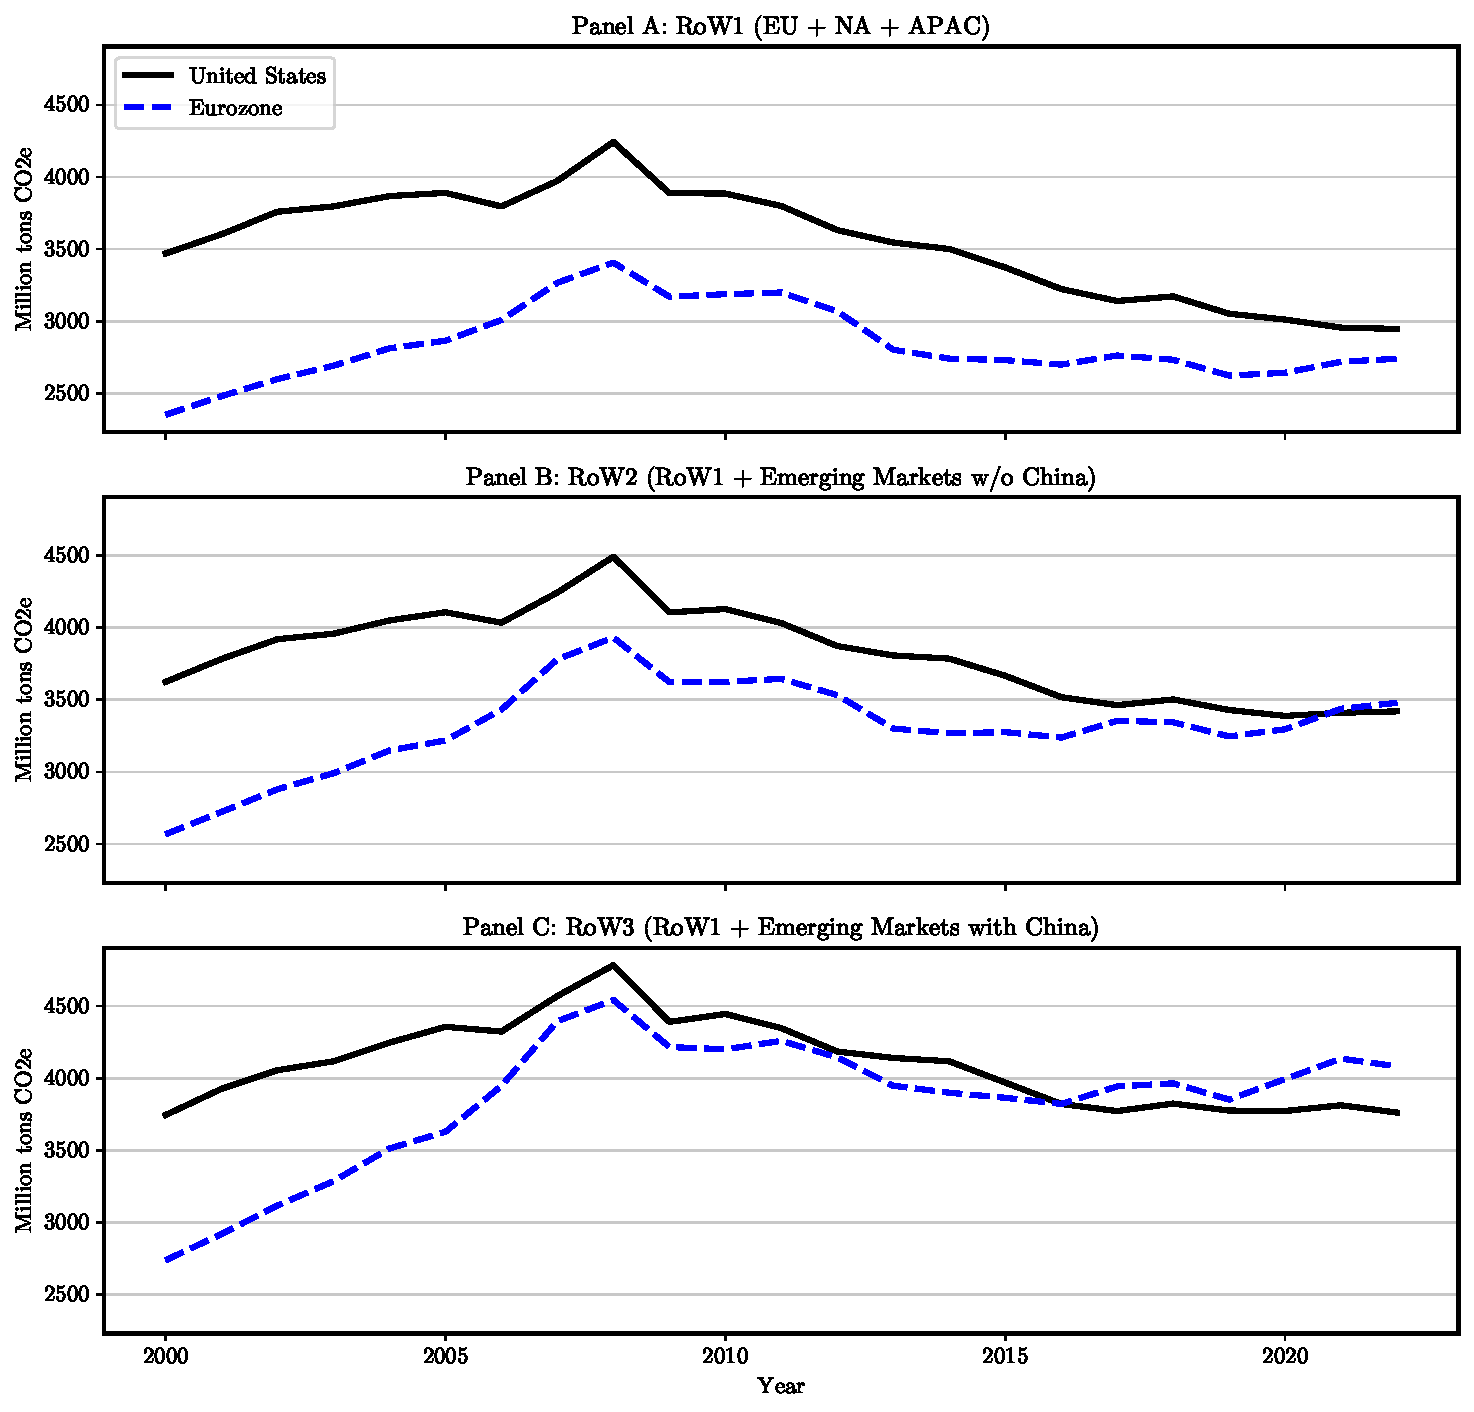
\includegraphics[width=1\textwidth]{Figures/US_vs_EU_By_Scenario_Vertical.pdf}
    \caption{Total financed emissions by RoW scenarios}
    \label{fig:total_financed_emis}
\end{figure}

Figure \ref{fig:total_financed_emis_fi} illustrates the breakdown of financed emissions across different types of financial institutions under the RoW1 scenario. Similar decompositions for the RoW2 and RoW3 scenarios are provided in the Appendix \ref{Appendix E:FE_by_FI}. The time-series patterns are broadly consistent across the three scenarios, suggesting that the relative evolution of financial institution groups is not sensitive to the choice of RoW allocation. The main difference is a vertical shift in the level of financed emissions: RoW2 and RoW3 generate higher estimates because they attribute a larger share of exposures to more carbon-intensive regions, particularly emerging markets and China. Thus, the alternative RoW assumptions primarily affect the scale of financed emissions, while leaving the composition and dynamics across financial institutions largely unchanged.

Consistent with the patterns identified in Figure \ref{fig:total_exp_fi}, the data indicates that structural market differences governing asset holdings serve as the primary driver of total financed emissions. A key observation is that investment funds account for the largest share of emissions in the US, stemming from their growing financial exposure to the domestic corporate sector. Conversely, in the Eurozone, Other Financial Institutions (OFIs) have generated emission levels comparable to those of Monetary Financial Institutions (MFIs) over the past decade, despite MFIs maintaining a significantly larger asset base. This parity is also largely driven by OFIs' increasing capital allocation toward emission-intensive non-financial corporations.
 
\begin{figure}[h]
    \centering
    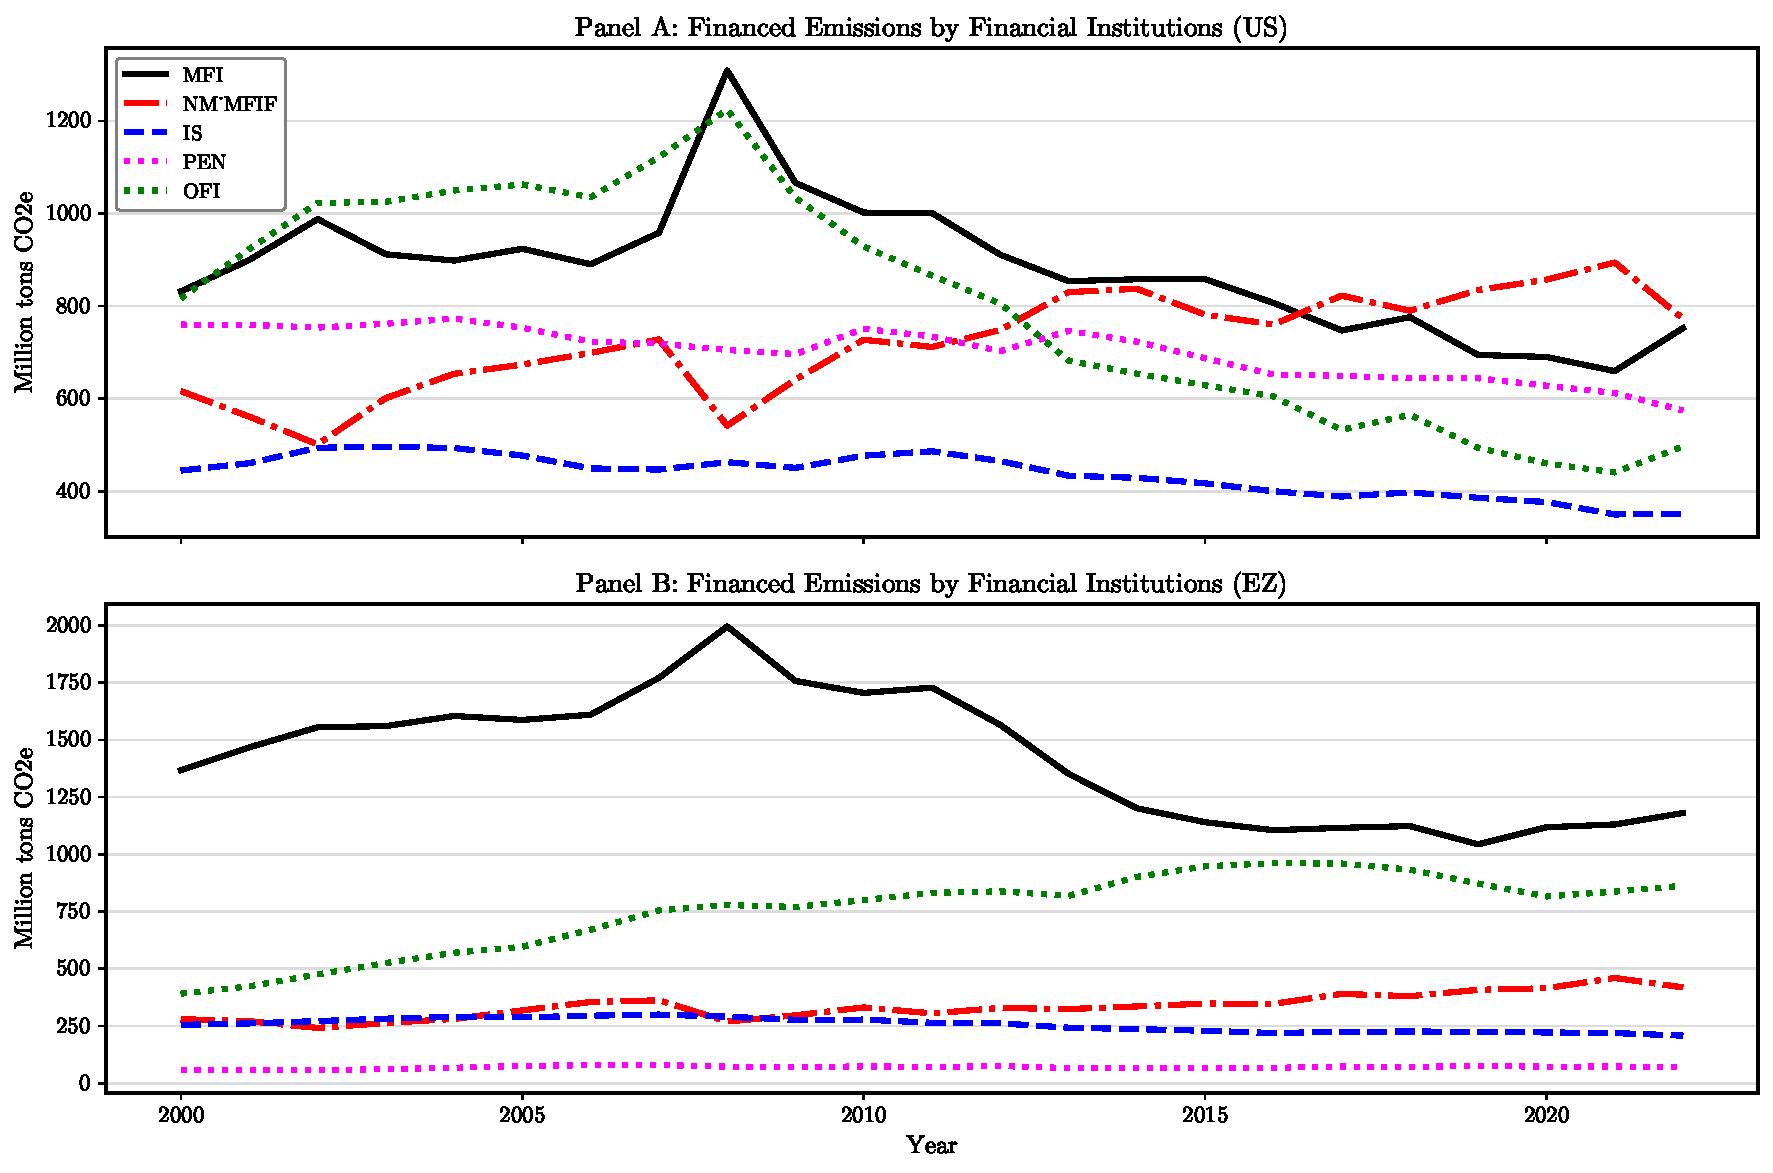
\includegraphics[width=1\textwidth]{Figures/FE_by_Institutions_RoW1.pdf}
    \caption{Total financed emissions by financial institution groups (RoW1)}
    \label{fig:total_financed_emis_fi}
\end{figure}

Figure~\ref{fig:total_financed_emis_agent} breaks down total financed GHG emissions by real-economy agents. The data reveals a profound structural divergence between the asset allocation strategies and environmental footprints of the two regions. The emissions profile of the United States financial system is characterized by an intense domestic focus and a steady long-term decline. Financed emissions are structurally dominated by domestic corporations, matching the US market-based framework where large capital-funded pension and investment fund structures allocate capital heavily into domestic securities markets. Total financed emissions have steadily contracted from their 2008 peak of approximately 3,083 million tonnes $\text{CO}_2\text{e}$. Furthermore, the cross-border layers ($\text{RoW1}$, $\text{RoW2}$, and $\text{RoW3}$) remain tight and visually compressed at the top of the stack, implying that the overall carbon footprint of the US financial sector is highly sensitive to domestic corporate decarbonization rather than international portfolio rebalancing.

In contrast, the Euro area panel exposes a structural migration of financed environmental pressures from domestic to cross-border domains. Following the dual shocks of the 2008 Global Financial Crisis and the 2012 Eurozone sovereign debt crisis, the financed emissions footprint of domestic European corporations contracted. However, this domestic compression was systematically offset by an aggressive expansion of cross-border claims. 

As the analytical lens moves sequentially from developed foreign portfolios ($\text{RoW1}$) to emerging markets ($\text{RoW2}$) and ultimately integrates China ($\text{RoW3}$), the Eurozone's total portfolio emissions experience a massive vertical shift. This visual transformation strongly supports the hypothesis that the Euro area financial system has actively outsourced its ecological footprint; driven by internal regulatory and monetary pressures, European financial intermediaries executed an international search for yield that has anchored European capital to highly carbon-intensive production networks abroad.

\begin{figure}[h]
    \centering
    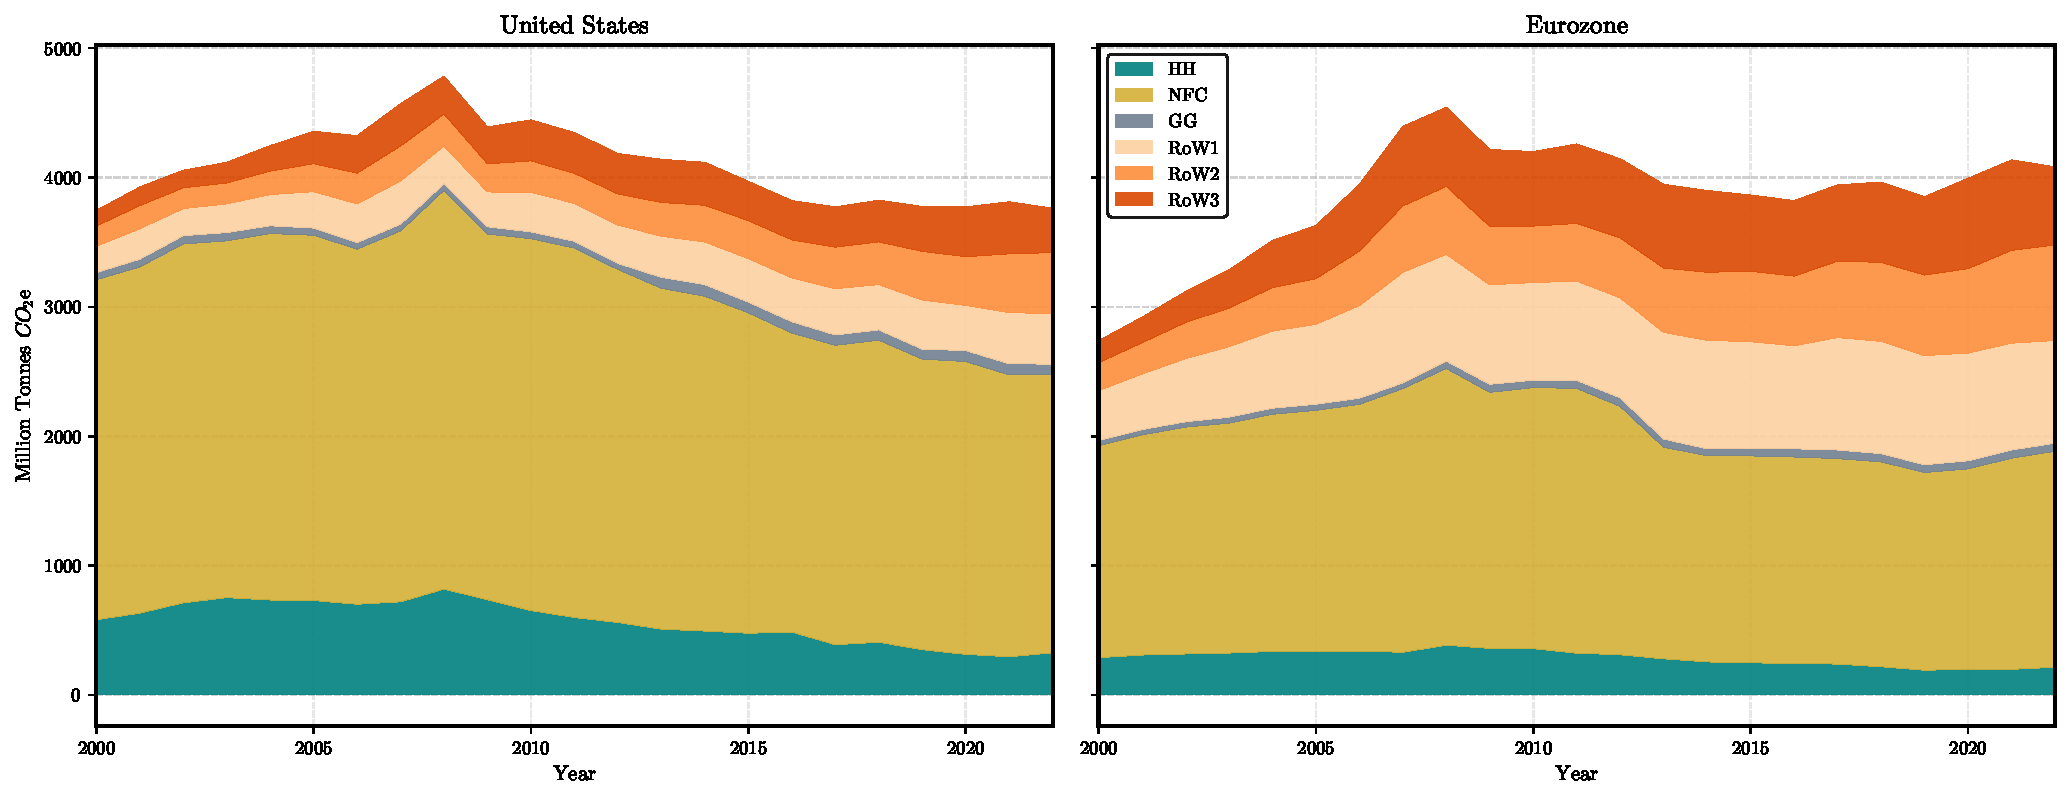
\includegraphics[width=1\textwidth]{Figures/FE_by_Agent.pdf}
    \caption{Total financed emissions by real-economy agents}
    \label{fig:total_financed_emis_agent}
\end{figure}

Figure \ref{fig:fe_cba_pba} compares the range of financed emissions (across three RoW scenarios), against two standard accounting benchmarks: production-based emissions and consumption-based emissions. PBA reflects emissions generated directly by domestic production activities within a territory, whereas CBA captures the global emissions driven by domestic final demand. Over the last two decades, PBA and CBA in both the US and the Eurozone have experienced a decline, though the reduction has been minimal. However, the absolute magnitude of emissions in the US is substantially higher, nearly double that of the Eurozone. While this partly reflects economic scale, it also suggests the US lags behind the Eurozone in its decarbonization trajectory. Furthermore, CBA consistently exceeds PBA in both regions, indicating a net importation of carbon embodied in foreign goods and services.
\begin{figure}[h]
    \centering
    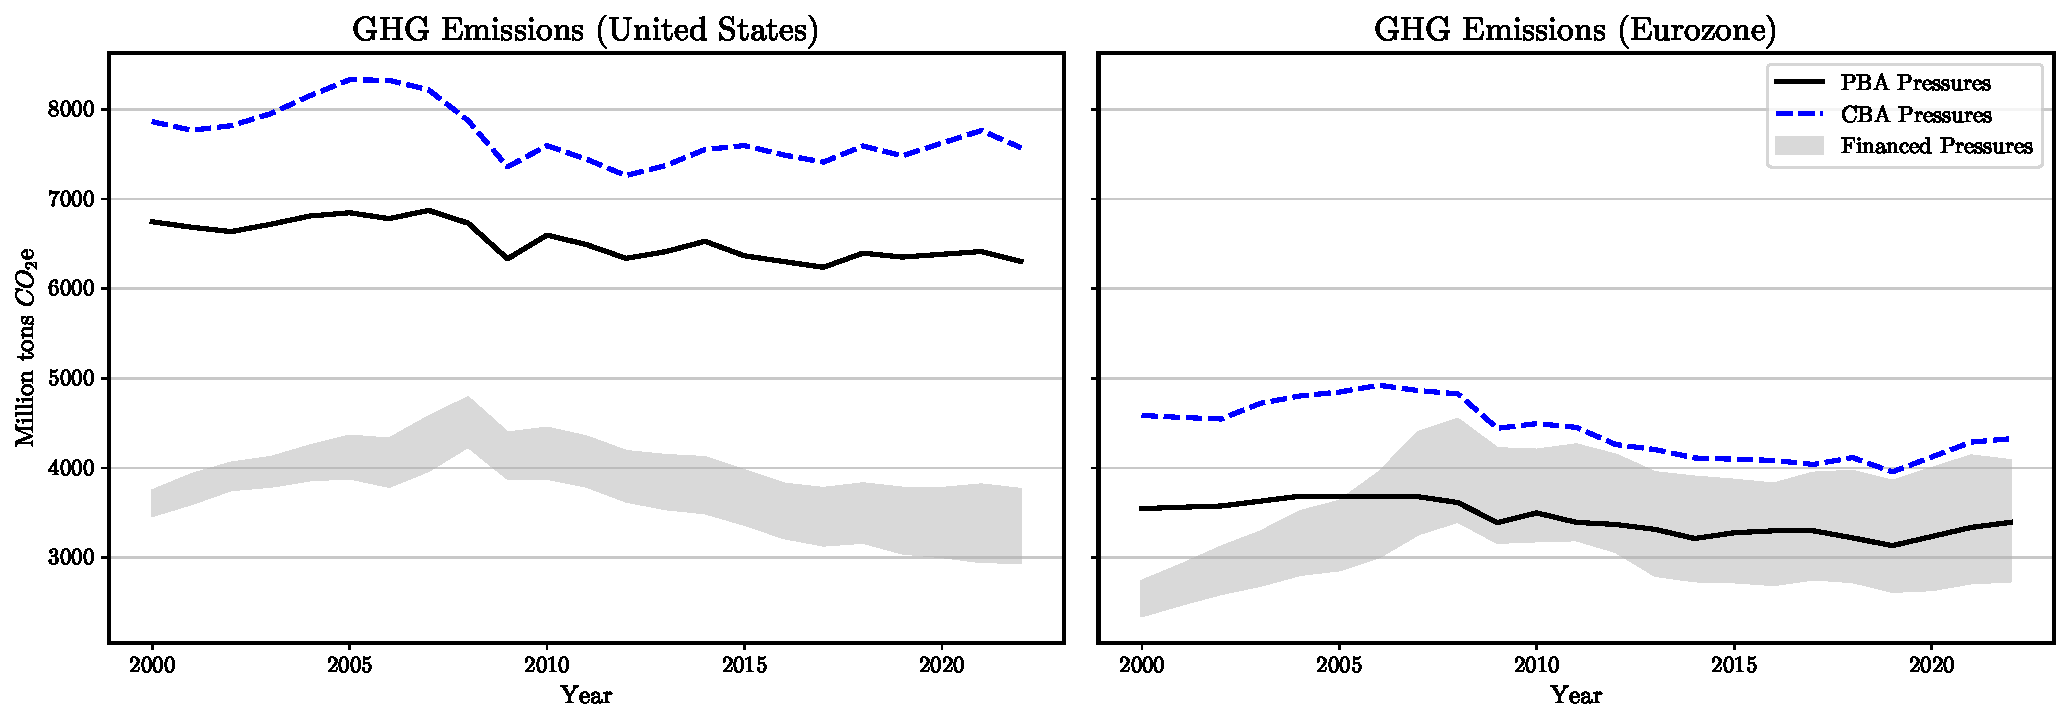
\includegraphics[width=1\textwidth]{Figures/Combined_FE_vs_PBA_CBA_GHG_emissions_GWP100_IPCC2010.pdf}
    \caption{Financed emissions in comparison with production-based and consumption-based emissions}
    \label{fig:fe_cba_pba}
\end{figure}

Interestingly, the relative significance of financed emissions diverges sharply between the two economies. In the US, although absolute financed emissions are substantial, they represent a smaller fraction of the overall carbon profile compared to massive domestic physical emissions. Conversely, in the Eurozone, the estimated range of financed emissions is roughly equivalent to the region's entire territorial (PBA) and demand-driven (CBA emissions. This highlights the disproportionately large global carbon footprint of the European financial sector relative to its domestic real economy.

\section{Other environmental pressures and resource use}
\label{sec:6.3}

In this section, the analysis is extended to other environmental pressures directly linked to the production activities enabled by financial system in the US and the Eurozone. Specifically, I consider land use, water consumption and the extraction of key material resources. The objective is to quantify how financial exposures translate into primary physical pressures on ecosystems and natural resources. 

\subsection{Land use and water consumption}

According to \textcite{stadler_exiobase_2018}, EXIOBASE considers three land-use categories: cropland, grazing land, and forestland. Cropland captures land used for crop production, grazing land refers to land used for pasture and livestock-related activities, and forestland captures land associated with forestry and timber-related production. In this thesis, the term ''land use'' refers to the aggregate of these three categories, representing the overall land-related pressure associated with economic activity.

Figure \ref{fig:land_use} compares production-based, consumption-based, and financed land-use pressures for the United States and the Eurozone. In both regions, consumption-based pressures are consistently higher than production-based pressures, suggesting that domestic consumption relies on land-intensive production outside the domestic economy. The United States exhibits substantially larger land-use pressures than the Eurozone across all accounting approaches. For the United States, financed land-use pressures remain relatively stable below both PBA and CBA measures. In contrast, financed land-use pressures in the Eurozone are closer to domestic production-based pressures and exceed them for most of the sample period. This indicates that, while Eurozone territorial land-use pressures are relatively limited, its financial system is associated with a broader land-use footprint through cross-border financial exposures. Overall, the figure highlights that financial-system-based accounting provides a distinct perspective from both production- and consumption-based measures, especially for economies with different financial structures and international exposure patterns.

\begin{figure}[h]
    \centering
    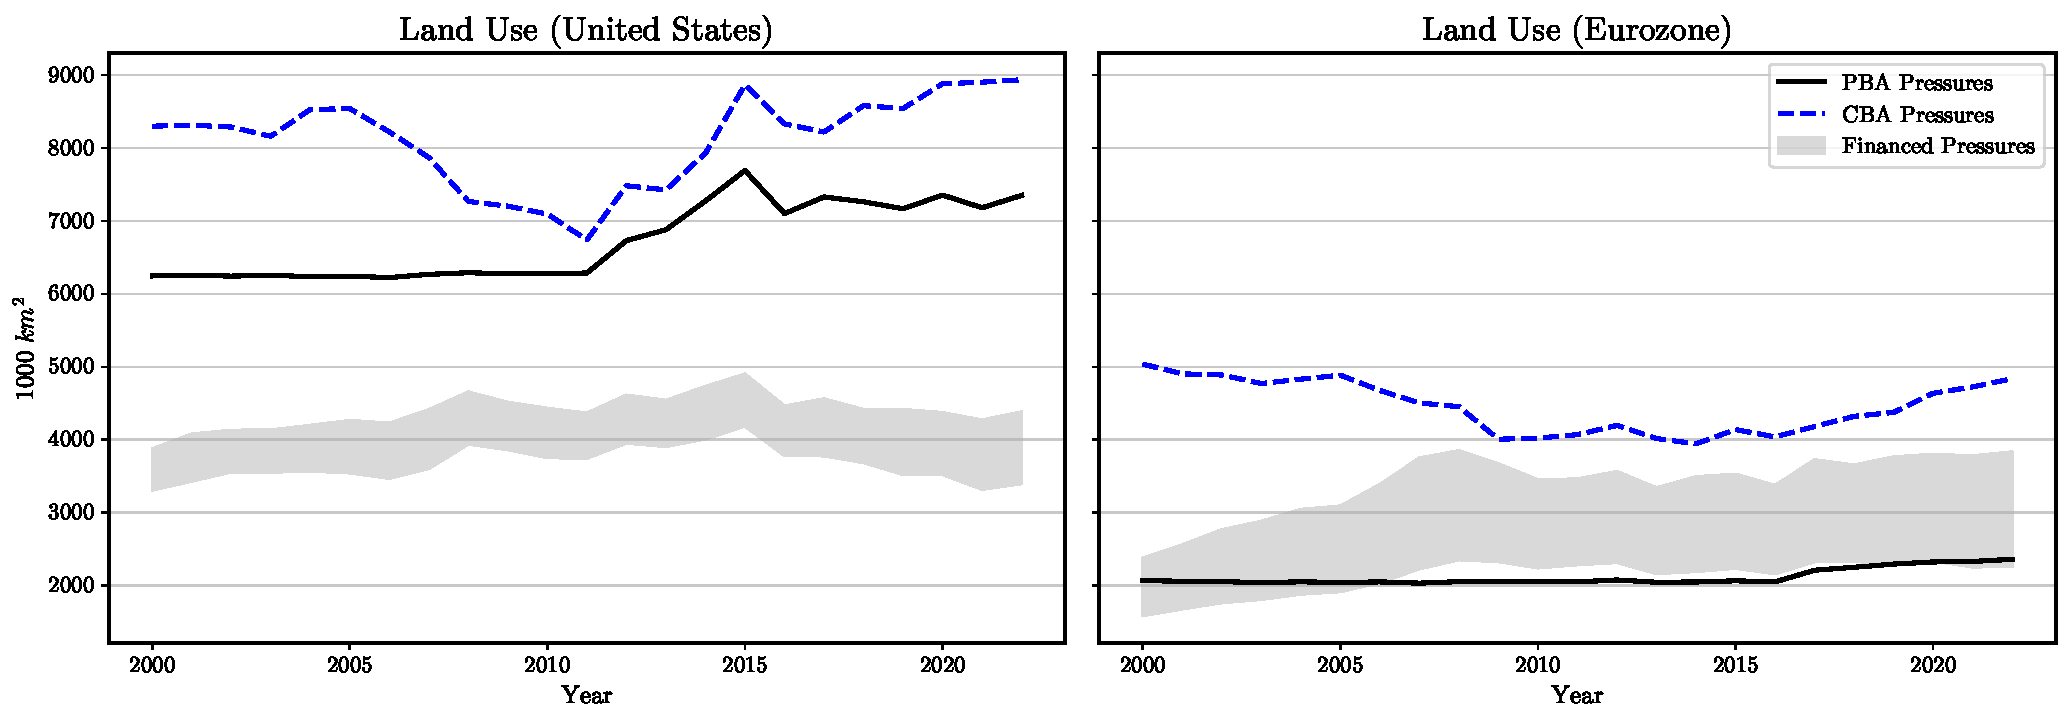
\includegraphics[width=1\textwidth]{Figures/Combined_FE_vs_PBA_CBA_Land_use_Crop_Forest_Pasture.pdf}
    \caption{Financed pressures in comparison with production-based and consumption-based pressures (Land Use in 1000 $km^2$)}
    \label{fig:land_use}
\end{figure}

Water-related accounts in EXIOBASE distinguish between green and blue water, as well as between water withdrawal and water consumption. The hydrological cycle is composed of both blue and green water. Blue water refers to the share of precipitation that flows into aquifers, lakes, rivers, and other surface-water and groundwater resources \citep{savenije_water_2000}. It is the main source of water for human needs, industrial production, and irrigated agriculture \citep{dantas_economic_2021}. Green water refers to the part of precipitation that is intercepted by vegetation, stored in the soil, transpired back to the atmosphere, or temporarily available for vegetation growth \citep{quinteiro_contribution_2015}. It plays a central role in agricultural production and is estimated to support around 60--70\% of global food production \citep{rost_agricultural_2008}.

Water withdrawal refers to the amount of water removed from natural sources and allocated to human activities \citep{gleick_water_2003, rijsberman_water_2006}. However, part of the withdrawn water may return to the natural water system before or after production processes. By contrast, water consumption refers to the portion of water that is consumed during production or use and does not return to the same hydrological system. Compared with water withdrawal, water consumption therefore provides a closer measure of water depletion and of the effective environmental pressure placed on freshwater resources. In this thesis, water pressure is measured using total blue water consumption, which aggregates blue water consumed across the main EXIOBASE activity categories, including agriculture, livestock production, electricity generation, manufacturing, and domestic use.

Figure \ref{fig:water_use} compares production-based, consumption-based, and financed pressures for total blue water consumption. In both the United States and the Euro area, consumption-based pressures exceed production-based pressures, indicating that both economies are net importers of blue-water consumption through international trade. However, the size of this gap differs substantially across the two regions. In the United States, CBA and PBA pressures remain relatively close to each other throughout the sample period, suggesting that foreign embodied water use plays a more limited role relative to domestic water consumption. By contrast, the Euro area shows a much larger and more persistent gap: production-based pressures remain relatively stable at around 40 billion m$^3$, while consumption-based pressures are roughly twice as large. This indicates that the Euro area relies more heavily on water-intensive production taking place outside its own territorial boundary.

The role of financed water pressures also differs between the two financial systems. In the United States, financed pressures remain clearly below both PBA and CBA measures, implying that financial-system exposures account for a relatively smaller share of the economy's overall blue-water footprint. In the Euro area, financed pressures are much closer to consumption-based pressures and rise above both PBA and CBA measures towards the end of the sample. This suggests that, compared with the United States, the Euro area financial system is more strongly linked to water-intensive real-economy activities through cross-border financial claims. Overall, the figure shows that both economies are net importers of water pressure, but the external dependence is more pronounced for the Euro area, where financial exposures also play a more important role in shaping the aggregate water footprint.

\begin{figure}[h]
    \centering
    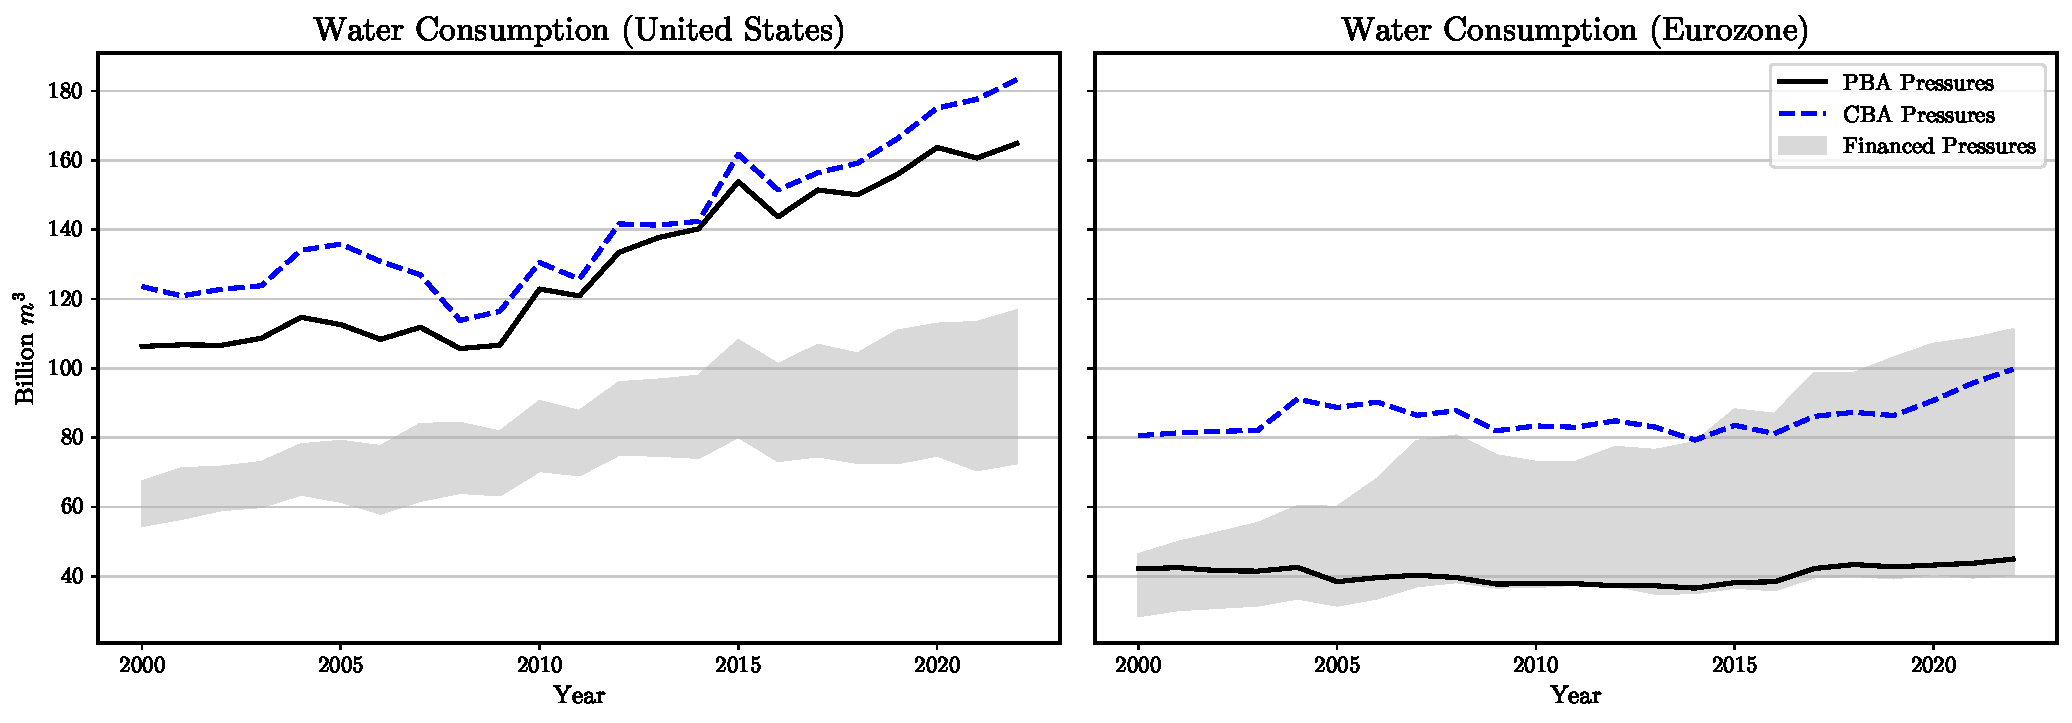
\includegraphics[width=1\textwidth]{Figures/Combined_FE_vs_PBA_CBA_Water_Consumption_Blue_Total.pdf}
    \caption{Financed pressures in comparison with production-based and consumption-based pressures (Water Consumption in billions $m^3$)}
    \label{fig:water_use}
\end{figure}

\subsection{Resource Extraction}

Resource extraction provides another dimension of environmental pressure associated with economic activity. In EXIOBASE, material extraction includes fossil fuels, iron ore, non-ferrous metal ores, and non-metallic minerals. These resources are tightly linked to different segments of the global production system. Fossil fuels are closely related to primary energy consumption, electricity generation, and carbon-intensive manufacturing processes. Iron ore serves as the foundational upstream raw material required for global steel production, linking it directly to heavy industrial manufacturing, machinery fabrication, and large-scale engineering projects. Non-ferrous metal ores, such as copper and aluminum, represent critical inputs for advanced engineering, electronics, and specialized industrial supply chains. Finally, non-metallic minerals, including sand, gravel, and limestone, are largely consumed by construction and infrastructure-related activities. Unlike GHG emissions, which measure an undesirable output of production, resource extraction captures the upstream, primary physical material requirements needed to sustain economic production and consumption.

Figure \ref{fig:resource_extraction_all} compares production-based, consumption-based, and financed pressures for four categories of resource extraction. Across most categories, consumption-based pressures exceed production-based pressures, indicating that both the United States and the Euro area rely on material extraction embodied in imported goods and foreign production chains. However, this dependence is more pronounced for the Euro area. In the United States, domestic extraction remains relatively important, especially for fossil fuels and non-metallic minerals, so the gap between production-based and consumption-based pressures is generally moderate. By contrast, the Euro area displays a larger and more systematic gap between consumption-based and production-based pressures, particularly for fossil fuels, non-ferrous metal ores, and iron ore. This suggests that the Euro area's material footprint is more strongly shaped by extraction taking place outside its territorial boundary.

The financed-pressure measure further highlights the difference between the two financial systems. In the United States, financed resource-extraction pressures generally remain below production-based and consumption-based pressures, suggesting that financial-system exposures play a relatively smaller role in the US material footprint. In the Euro area, financed pressures are closer to consumption-based pressures and often exceed production-based pressures, especially for metal ores. This indicates that Euro area financial institutions are linked to resource-intensive activities that largely take place abroad. Overall, the figure shows that both economies are net importers of material pressures through trade, but the external dependence is stronger for the Euro area. 

\begin{figure}[htbp]
    \centering
    \begin{tabular}{c}
        % ==================== CHART 1 ====================
        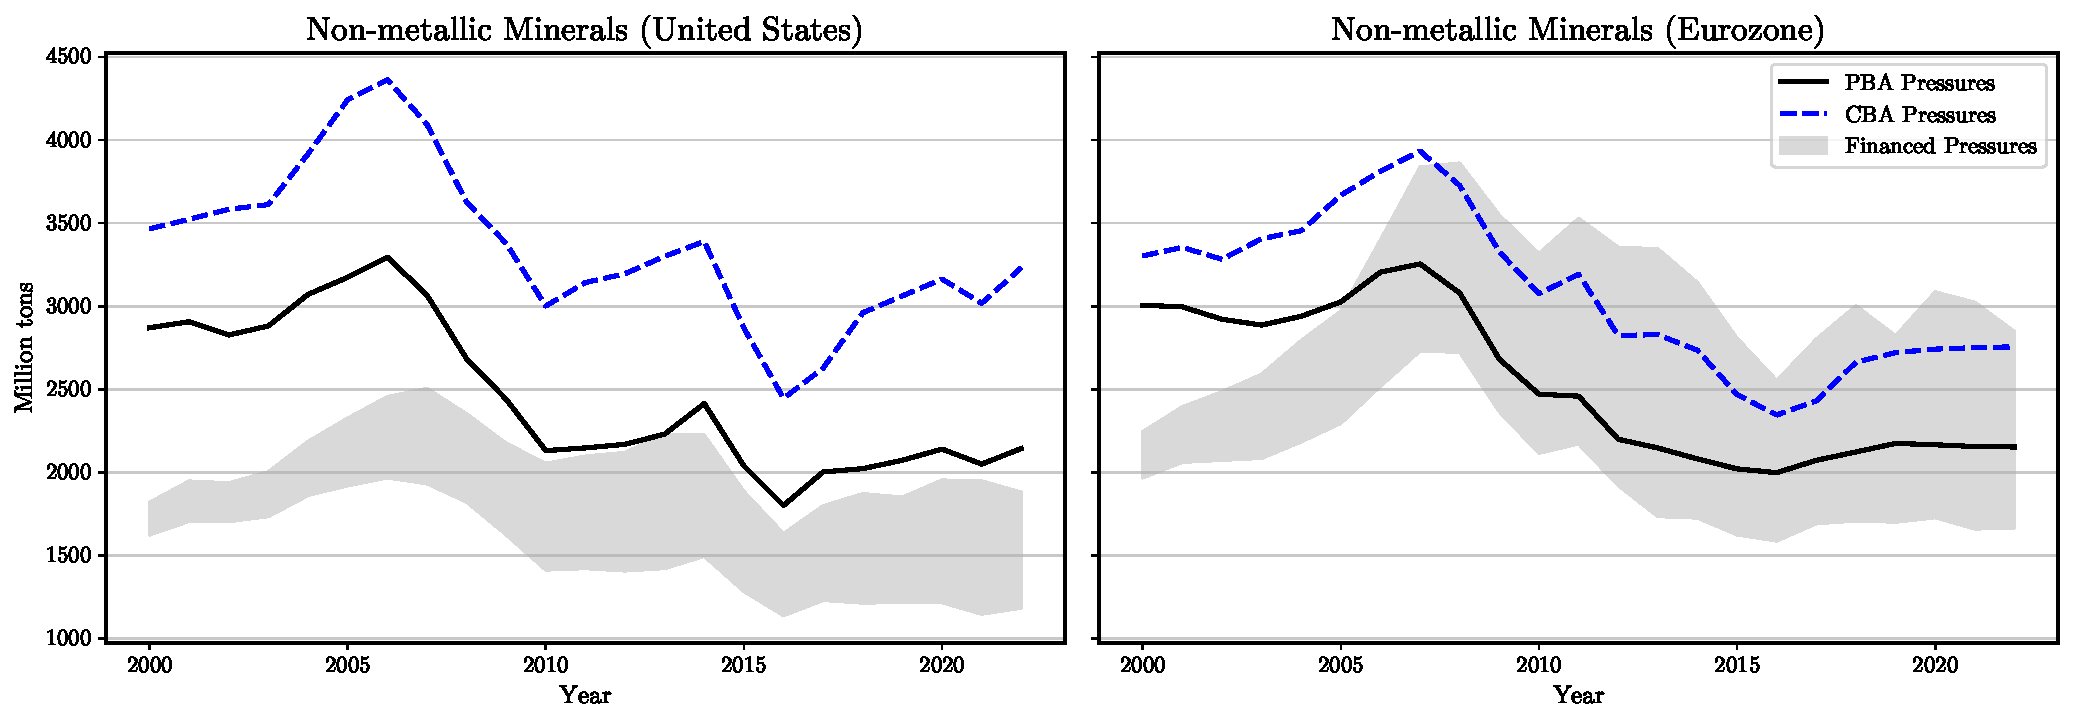
\includegraphics[width=0.9\textwidth]{Figures/Combined_FE_vs_PBA_CBA_DEU_Non_metalic_Minerals.pdf}\\
        
        % ==================== CHART 2 ====================
        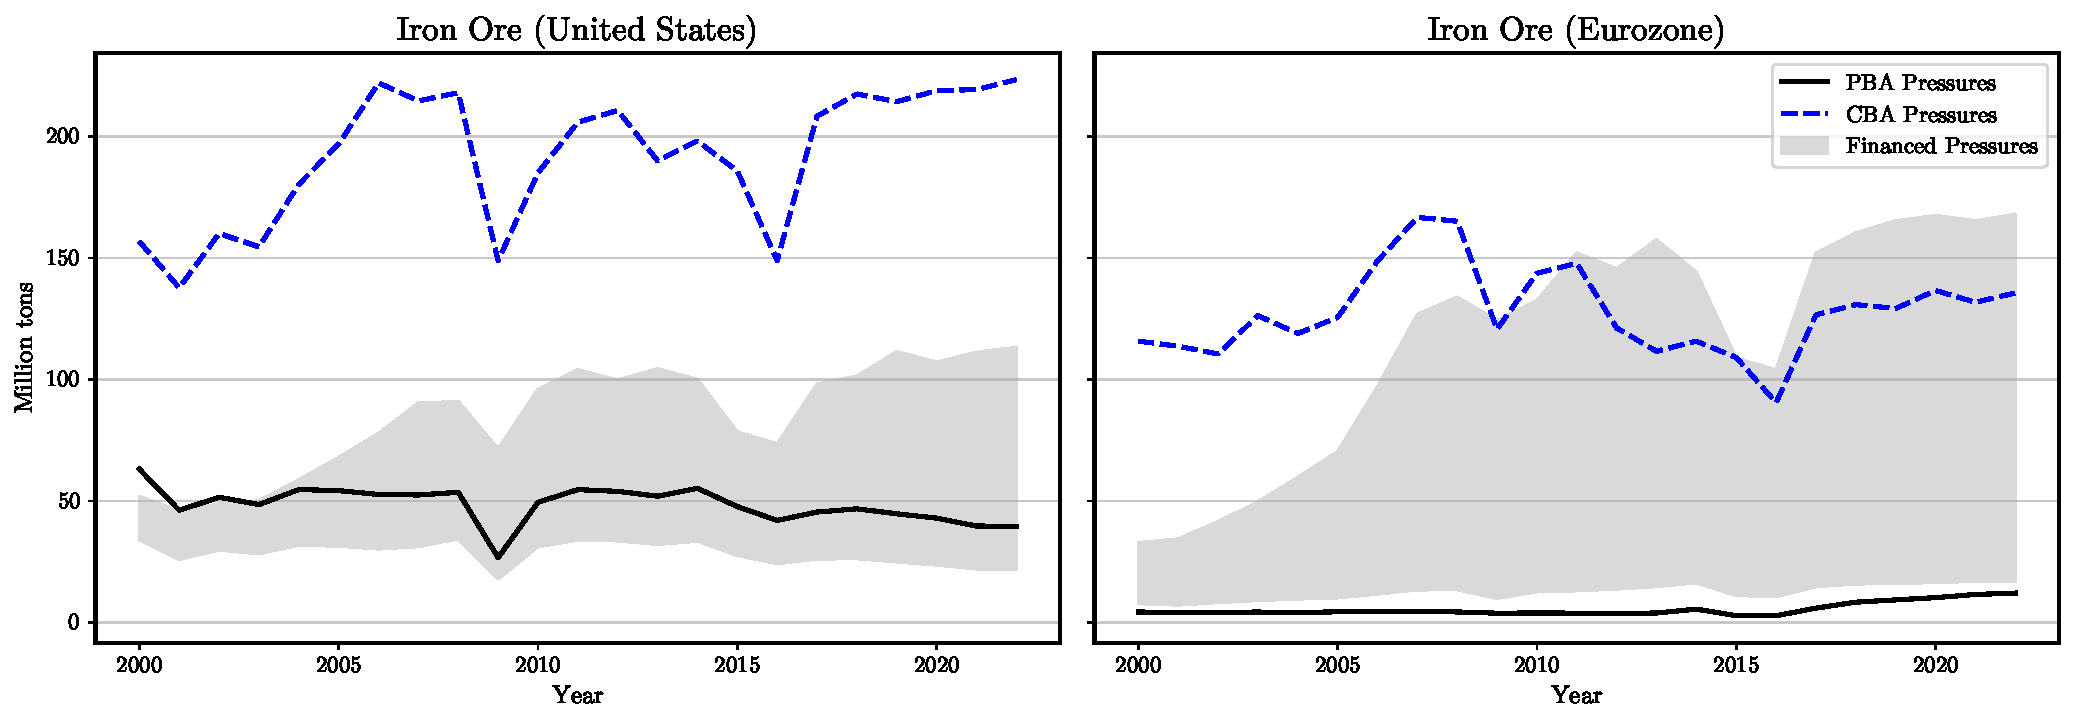
\includegraphics[width=0.9\textwidth]{Figures/Combined_FE_vs_PBA_CBA_DEU_Iron_Ore.pdf} \\
        
        % ==================== CHART 3 ====================
        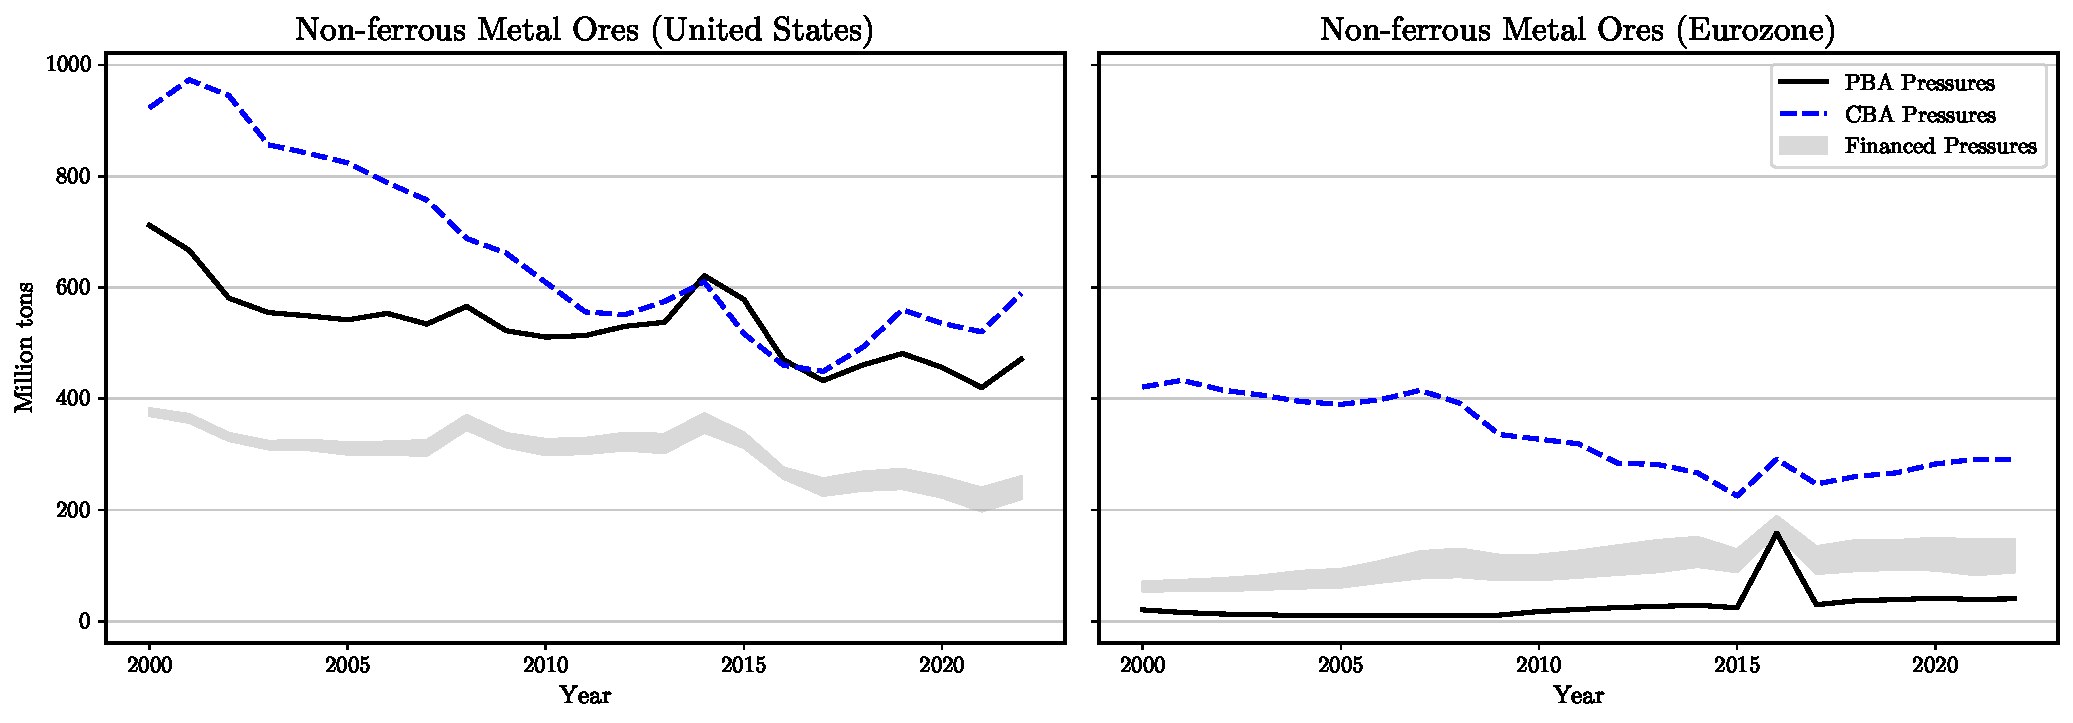
\includegraphics[width=0.9\textwidth]{Figures/Combined_FE_vs_PBA_CBA_DEU_Non_ferous_metal_ores.pdf} \\
        
        % ==================== CHART 4 ====================
        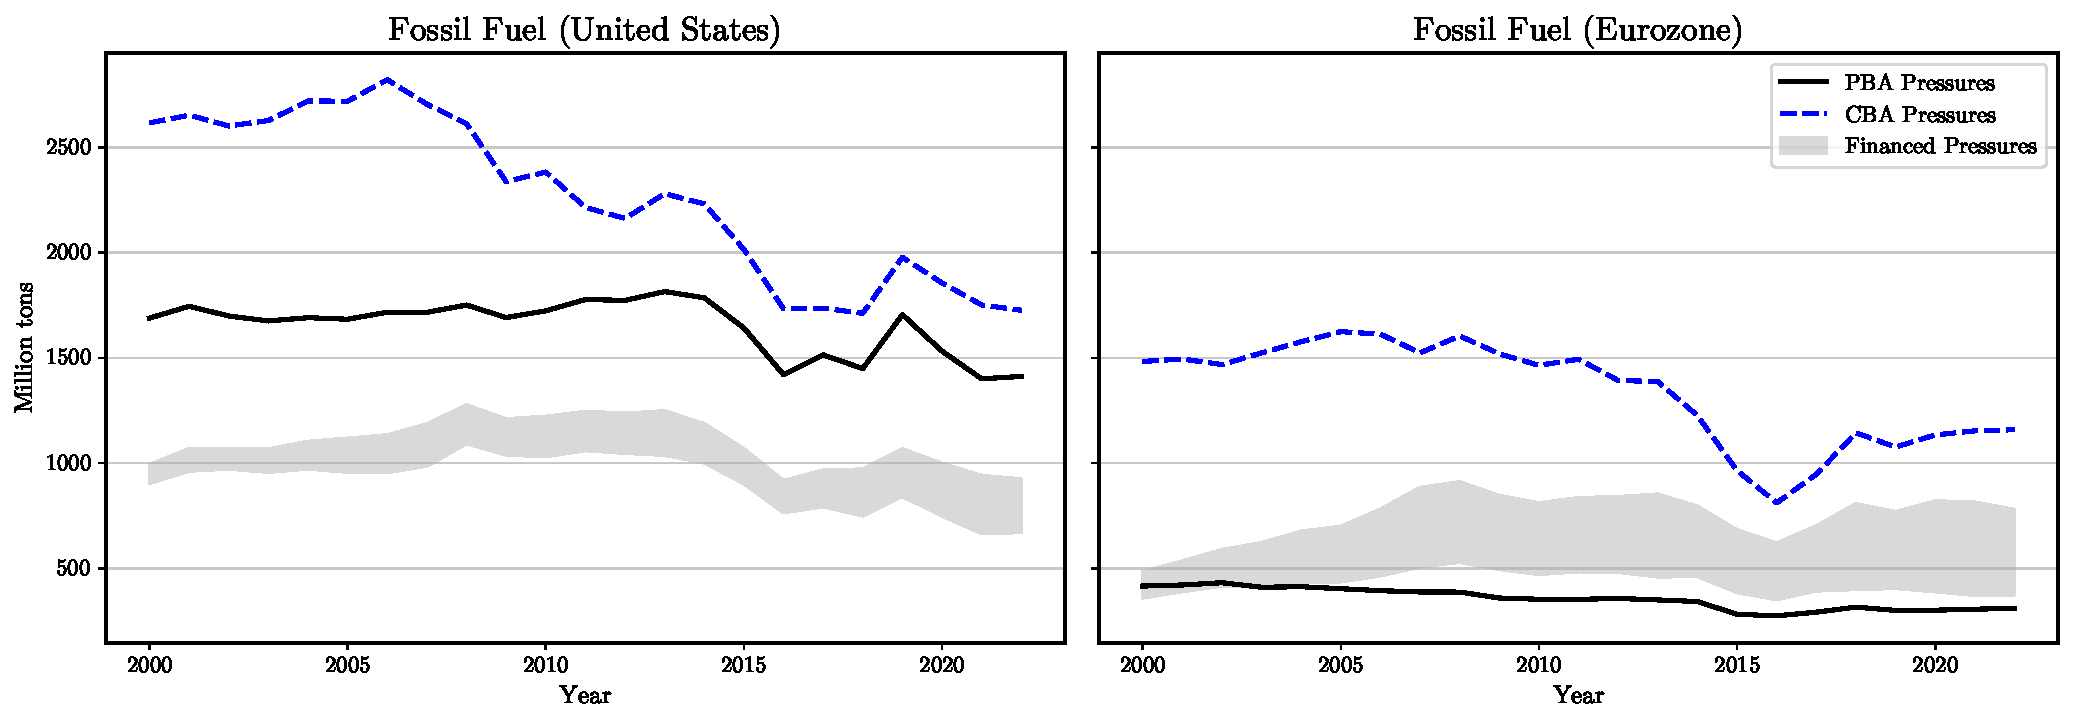
\includegraphics[width=0.9\textwidth]{Figures/Combined_FE_vs_PBA_CBA_DEU_Fossil_Fuel.pdf} \\
    \end{tabular}

    % ==================== MAIN CAPTION ====================
    \caption{Financed pressures in comparison with production-based and consumption-based pressures for Resource Extraction variants (Physical Units in Million tons).}
    \label{fig:resource_extraction_all}
\end{figure}